\documentclass{article}

\usepackage{tikz} 
\usetikzlibrary{automata, positioning, arrows} 

\usepackage{amsthm}
\usepackage{amsfonts}
\usepackage{amsmath}
\usepackage{amssymb}
\usepackage{fullpage}
\usepackage{color}
\usepackage{parskip}
\usepackage{hyperref}
  \hypersetup{
    colorlinks = true,
    urlcolor = blue,       % color of external links using \href
    linkcolor= blue,       % color of internal links 
    citecolor= blue,       % color of links to bibliography
    filecolor= blue,        % color of file links
    }
    
\usepackage{listings}

\definecolor{dkgreen}{rgb}{0,0.6,0}
\definecolor{gray}{rgb}{0.5,0.5,0.5}
\definecolor{mauve}{rgb}{0.58,0,0.82}

\lstset{frame=tb,
  language=haskell,
  aboveskip=3mm,
  belowskip=3mm,
  showstringspaces=false,
  columns=flexible,
  basicstyle={\small\ttfamily},
  numbers=none,
  numberstyle=\tiny\color{gray},
  keywordstyle=\color{blue},
  commentstyle=\color{dkgreen},
  stringstyle=\color{mauve},
  breaklines=true,
  breakatwhitespace=true,
  tabsize=3
}

\newtheoremstyle{theorem}
  {\topsep}   % ABOVESPACE
  {\topsep}   % BELOWSPACE
  {\itshape\/}  % BODYFONT
  {0pt}       % INDENT (empty value is the same as 0pt)
  {\bfseries} % HEADFONT
  {.}         % HEADPUNCT
  {5pt plus 1pt minus 1pt} % HEADSPACE
  {}          % CUSTOM-HEAD-SPEC
\theoremstyle{theorem} 
   \newtheorem{theorem}{Theorem}[section]
   \newtheorem{corollary}[theorem]{Corollary}
   \newtheorem{lemma}[theorem]{Lemma}
   \newtheorem{proposition}[theorem]{Proposition}
\theoremstyle{definition}
   \newtheorem{definition}[theorem]{Definition}
   \newtheorem{example}[theorem]{Example}
\theoremstyle{remark}    
  \newtheorem{remark}[theorem]{Remark}

\setcounter{tocdepth}{3}  % This makes subsubsections (level 3) appear in TOC
\setcounter{secnumdepth}{3}  % This makes subsubsections numbered
  

\title{CPSC-406 Report}
\author{Charlie Conner  \\ Chapman University}

\date{\today} 

\begin{document}

\maketitle

\begin{abstract}
This is the place to write an abstract. The abstract should be a short summary of the report. It should be written in a way that makes it possible to understand the purpose of the report without reading it. You can write a dummy abstract first and replace it with a real one later in the semester.
\end{abstract}

\setcounter{tocdepth}{3}
\tableofcontents

\section{Introduction}\label{intro}

This report will document your learning throughout the course. It will be a collection of your notes, homework solutions, and critical reflections on the content of the course. Something in between a semester-long take home exam and your own lecture notes.\footnote{One purpose of giving the report the form of lecture notes is that self-explanation is a technique proven to help with learning, see Chapter 6 of Craig Barton, How I Wish I'd Taught Maths, and references therein. In fact, the report can lead you from self-explanation (which is what you do for the weekly deadline) to explaining to others (which is what you do for the final submission). Another purpose is to help those of you who want to go on to graduate school to develop some basic writing skills. A report that you could proudly add to your application to graduate school (or a job application in industry) would give you full points.}

To write your own report, you start from \texttt{report.tex} which is available in the course repo. For guidance on how to do this read on and also consult \texttt{latex-example.tex} which is also available in the repo. Also check out the usual resources (Google, Stackoverflow, LLM, etc). It was never as easy as now to learn a new programming lanugage (which, btw, \LaTeX{} is).

For writing \LaTeX{} with VSCode, consider using the \href{https://marketplace.visualstudio.com/items?itemName=James-Yu.latex-workshop}{\LaTeX{} Workshop} extension. 

There will be deadlines during the semester, graded mostly for completeness. That means that you will get the points if you submit in time and are on the right track, independently of whether the solutions are technically correct. You will have the opportunity to revise your work for the final submission of the full report.

The full report is due at the end of the finals week. It will be graded according to the following guidelines.

Grading  guidelines (see also below):
\begin{itemize}
\item Is typesetting and layout professional? 
\item Is the technical content, in particular the homework, correct?
\item Did the student find interesting references~\cite{bla} and cites them throughout the report?
\item Do the notes reflect understanding and critical thinking?
\item Does the report contain material related to but going beyond what we do in class?
\item Are the questions interesting?
\end{itemize}

Do not change the template (fontsize, width of margin, spacing of lines, etc) without asking your first.

\section{Week by Week}\label{homework}

\subsection{Week 0 (EXAMPLE)}

Week 1 aligns with the first week of the semester. 

If you think that the writing flows better if you merge the sections ``Notes'' and ``Homework'', you can do so, but keep the heading for ``Comments and Questions''.

\subsubsection{Notes}

This section is optional. 

Our experience is that writing notes is a great way to learn. You can use this section to write your own notes and showcase your own understanding. 

\subsubsection{Homework}

This section will typically contain Homework problems. You should write up your solutions in \LaTeX{}. You can use the \texttt{lstlisting} environment to include code. You can use \href{https://excalidraw.com/}{Excalidraw} for drawings. Pictures from handwritten drawings are acceptable if the drawings are of high quality (pictures from rough notes and quick sketches are likely to loose you points). 

Make sure that this section can be read without referring back to the homework question. Introduce the question/problem and repeat it in your own words. Make sure to typset your homework in a way that makes it clear what  the question and what the answer is. Present it as a worked example would be presented in a textbook. 

Also explain what you learn from the homework. Each homework was carefully drafted to bring home a particular teaching point. Make sure to explain what this point is. Relate it to the big questions mentioned above. 

In case you want to draw automata in \LaTeX{}, you can use the tikz package. Here is an example of a simple automaton:

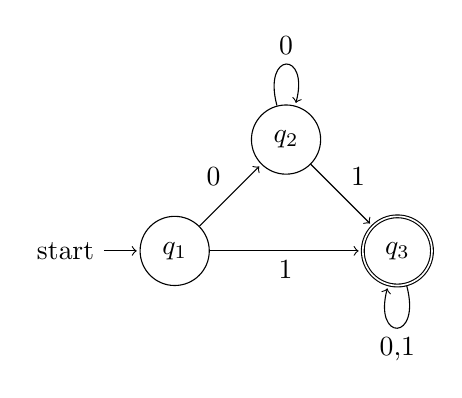
\begin{tikzpicture}[shorten >=1pt,node distance=2cm,on grid,auto] 
  % Define states
  \node[state, initial] (q_1)   {$q_1$};  % q1 is now the start state
  \node[state] (q_2) [above right=of q_1] {$q_2$}; 
  \node[state, accepting] (q_3) [below right=of q_2] {$q_3$};  % q3 is now the final state

  % Define transitions
  \path[->] 
    (q_1) edge  node {0} (q_2)
          edge  node [swap] {1} (q_3)
    (q_2) edge  node  {1} (q_3)
          edge [loop above] node {0} ()
    (q_3) edge [loop below] node {0,1} ();

\end{tikzpicture}

By the way, ChatGPT is quite good at outputting tikz code. Another alternative package is xymatrix.

\subsubsection{Exploration}

Here are some hints. Why is this material included in the course? What are the big questions that motivate the study of this subject? How does this material connect to broader themes or issues in the field? What practical or theoretical problems can be addressed through an understanding of these topics? A great way to test whether you understand the material is to make your own exercises and answer them. Material related to but going beyond what we do in class is welcome.

Feel free to use your favourite LLM to help you build a mental landscape of the subject. Think of LLMs as an extension of Wikipedia and Google, a tool you should be using as introduction to any subject. If you didn't check with Google, Wikipedia and GPT, you are not ready to write your own notes. On the other hand, while using these resources is necessary, you need to always exercise your own critical thinking and you are always responsible for what you write. 


\subsubsection{Questions}

Ask at least one \textbf{interesting question}\footnote{It is important to learn to ask \emph{interesting} questions. There is no precise way of defining what is meant by interesting. You can only learn this by doing. An interesting question comes typically in two parts. Part 1 (one or two sentences) sets the scene. Part 2 (one or two sentences) asks the question. A good question strikes the right balance between being specific and technical on the one hand and open ended on the other hand. A question that can be answered with yes/no is not an interesing question.} on the lecture notes. Also post the question on the Discord channel so that everybody can see and discuss the questions.

\clearpage
\subsection{Week 1}

\subsubsection{Notes}

This section is optional. 

\subsubsection{Homework}

\textbf{Exercise 1 (Word processing with DFAs).}
Given two DFAs $\mathcal{A}_1$ and $\mathcal{A}_2$ over $\Sigma = \{a, b\}$, determine which words are accepted/refused and describe the accepted languages.

\paragraph{DFA $\mathcal{A}_1$.} States $\{1, 2, 3, 4\}$, start state $1$, accepting state $3$:

\begin{center}
\begin{tabular}{c|cc}
 & $a$ & $b$ \\ \hline
$1$ & $2$ & $4$ \\
$2$ & $2$ & $3$ \\
$3$ & $2$ & $2$ \\
$4$ & $4$ & $4$ \\
\end{tabular}
\end{center}

\paragraph{DFA $\mathcal{A}_2$.} States $\{1, 2, 3\}$, start state $1$, accepting state $3$:

\begin{center}
\begin{tabular}{c|cc}
 & $a$ & $b$ \\ \hline
$1$ & $2$ & $1$ \\
$2$ & $3$ & $1$ \\
$3$ & $3$ & $1$ \\
\end{tabular}
\end{center}

\paragraph{Part 1: Tracing words.} For each word, I walked through the transition table one character at a time and recorded the states:

\begin{center}
\begin{tabular}{c|c|c|c|c}
$w$ & $\mathcal{A}_1$ trace & $\mathcal{A}_1$? & $\mathcal{A}_2$ trace & $\mathcal{A}_2$? \\ \hline
$aaa$ & $1 \to 2 \to 2 \to 2$ & No & $1 \to 2 \to 3 \to 3$ & Yes \\
$aab$ & $1 \to 2 \to 2 \to 3$ & Yes & $1 \to 2 \to 3 \to 1$ & No \\
$aba$ & $1 \to 2 \to 3 \to 2$ & No & $1 \to 2 \to 1 \to 2$ & No \\
$abb$ & $1 \to 2 \to 3 \to 2$ & No & $1 \to 2 \to 1 \to 1$ & No \\
$baa$ & $1 \to 4 \to 4 \to 4$ & No & $1 \to 1 \to 2 \to 3$ & Yes \\
$bab$ & $1 \to 4 \to 4 \to 4$ & No & $1 \to 1 \to 2 \to 1$ & No \\
$bba$ & $1 \to 4 \to 4 \to 4$ & No & $1 \to 1 \to 1 \to 2$ & No \\
$bbb$ & $1 \to 4 \to 4 \to 4$ & No & $1 \to 1 \to 1 \to 1$ & No \\
\end{tabular}
\end{center}

\paragraph{Part 2: Describing the languages.}

\textbf{$L(\mathcal{A}_1)$: Words that start with $a$ and end with an odd-length block of consecutive $b$'s.}

Starting with $b$ traps us in state $4$, so the word must start with $a$. After that, reading $a$ resets us to state $2$, and reading $b$ flips between states $2$ and $3$. So we accept when the number of $b$'s since the last $a$ is odd.

\textbf{$L(\mathcal{A}_2)$: Words that end with $aa$.}

Any $b$ resets us to state $1$, and $a$'s move us along $1 \to 2 \to 3$ (staying in $3$ on more $a$'s). So we accept when the word ends with two or more $a$'s.

\bigskip

\textbf{Exercise 2 (Designing DFAs).}
Design DFAs over $\Sigma = \{a,b\}$ for each of the following languages.

\paragraph{(a) All words ending with $ab$.} Three states: $q_0$ (no progress), $q_1$ (last char was $a$), $q_2$ (saw $ab$, accepting).

\begin{center}
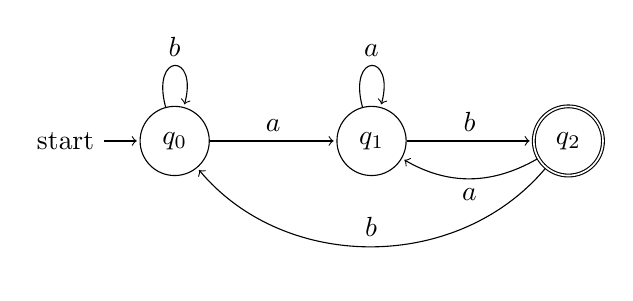
\begin{tikzpicture}[shorten >=1pt,node distance=2.5cm,on grid,auto]
  \node[state, initial] (q0) {$q_0$};
  \node[state] (q1) [right=of q0] {$q_1$};
  \node[state, accepting] (q2) [right=of q1] {$q_2$};
  \path[->]
    (q0) edge node {$a$} (q1)
         edge [loop above] node {$b$} ()
    (q1) edge node {$b$} (q2)
         edge [loop above] node {$a$} ()
    (q2) edge [bend left] node {$a$} (q1)
         edge [bend left=50] node [swap] {$b$} (q0);
\end{tikzpicture}
\end{center}

\paragraph{(b) All words containing $aba$.} Track how much of $aba$ we've matched. Once found, we stay accepting (trap state).

\begin{center}
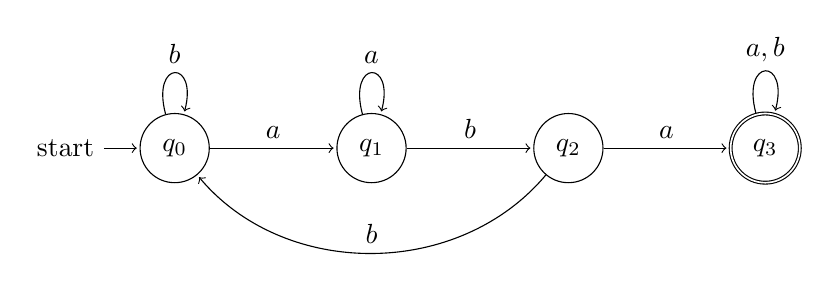
\begin{tikzpicture}[shorten >=1pt,node distance=2.5cm,on grid,auto]
  \node[state, initial] (q0) {$q_0$};
  \node[state] (q1) [right=of q0] {$q_1$};
  \node[state] (q2) [right=of q1] {$q_2$};
  \node[state, accepting] (q3) [right=of q2] {$q_3$};
  \path[->]
    (q0) edge node {$a$} (q1)
         edge [loop above] node {$b$} ()
    (q1) edge node {$b$} (q2)
         edge [loop above] node {$a$} ()
    (q2) edge node {$a$} (q3)
         edge [bend left=50] node [swap] {$b$} (q0)
    (q3) edge [loop above] node {$a,b$} ();
\end{tikzpicture}
\end{center}

\paragraph{(c) All words with an odd number of $a$'s and an odd number of $b$'s.} Four states for each combination of (parity of $a$'s, parity of $b$'s). Reading $a$ flips the $a$-parity, reading $b$ flips the $b$-parity.

\begin{center}
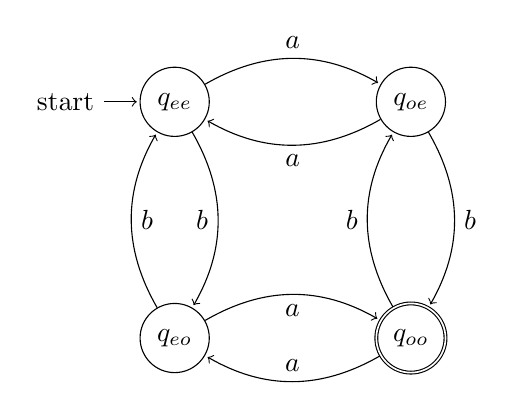
\begin{tikzpicture}[shorten >=1pt,node distance=3cm,on grid,auto]
  \node[state, initial] (ee) {$q_{ee}$};
  \node[state] (oe) [right=of ee] {$q_{oe}$};
  \node[state] (eo) [below=of ee] {$q_{eo}$};
  \node[state, accepting] (oo) [right=of eo] {$q_{oo}$};
  \path[->]
    (ee) edge [bend left] node {$a$} (oe)
         edge [bend left] node [swap] {$b$} (eo)
    (oe) edge [bend left] node {$a$} (ee)
         edge [bend left] node {$b$} (oo)
    (eo) edge [bend left] node [swap] {$b$} (ee)
         edge [bend left] node [swap] {$a$} (oo)
    (oo) edge [bend left] node {$b$} (oe)
         edge [bend left] node [swap] {$a$} (eo);
\end{tikzpicture}
\end{center}

\paragraph{(d) All words with an even number of $a$'s and an odd number of $b$'s.} Same DFA as (c), just with $q_{eo}$ as the accepting state instead of $q_{oo}$.

\begin{center}
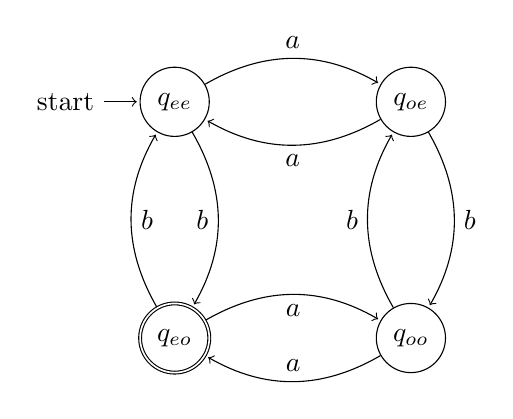
\begin{tikzpicture}[shorten >=1pt,node distance=3cm,on grid,auto]
  \node[state, initial] (ee) {$q_{ee}$};
  \node[state] (oe) [right=of ee] {$q_{oe}$};
  \node[state, accepting] (eo) [below=of ee] {$q_{eo}$};
  \node[state] (oo) [right=of eo] {$q_{oo}$};
  \path[->]
    (ee) edge [bend left] node {$a$} (oe)
         edge [bend left] node [swap] {$b$} (eo)
    (oe) edge [bend left] node {$a$} (ee)
         edge [bend left] node {$b$} (oo)
    (eo) edge [bend left] node [swap] {$b$} (ee)
         edge [bend left] node [swap] {$a$} (oo)
    (oo) edge [bend left] node {$b$} (oe)
         edge [bend left] node [swap] {$a$} (eo);
\end{tikzpicture}
\end{center}

\paragraph{(e) All words where any three consecutive characters contain at least one $a$.} This is the same as saying the word never contains $bbb$. We count consecutive $b$'s.

\begin{center}
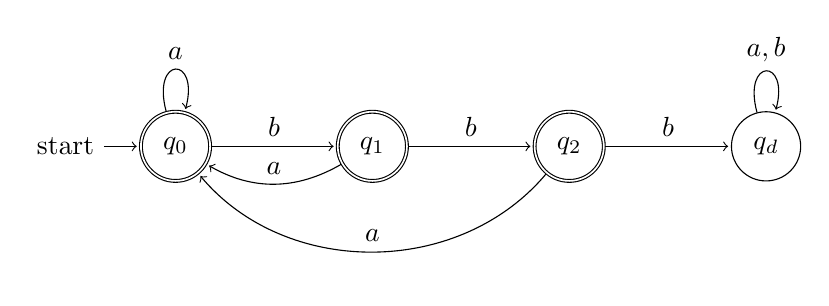
\begin{tikzpicture}[shorten >=1pt,node distance=2.5cm,on grid,auto]
  \node[state, initial, accepting] (q0) {$q_0$};
  \node[state, accepting] (q1) [right=of q0] {$q_1$};
  \node[state, accepting] (q2) [right=of q1] {$q_2$};
  \node[state] (qd) [right=of q2] {$q_d$};
  \path[->]
    (q0) edge node {$b$} (q1)
         edge [loop above] node {$a$} ()
    (q1) edge node {$b$} (q2)
         edge [bend left] node [swap] {$a$} (q0)
    (q2) edge node {$b$} (qd)
         edge [bend left=50] node [swap] {$a$} (q0)
    (qd) edge [loop above] node {$a,b$} ();
\end{tikzpicture}
\end{center}

\paragraph{(f) All words containing $bbb$.} Same idea as (e) but we count consecutive $b$'s until we hit three, then stay accepting.

\begin{center}
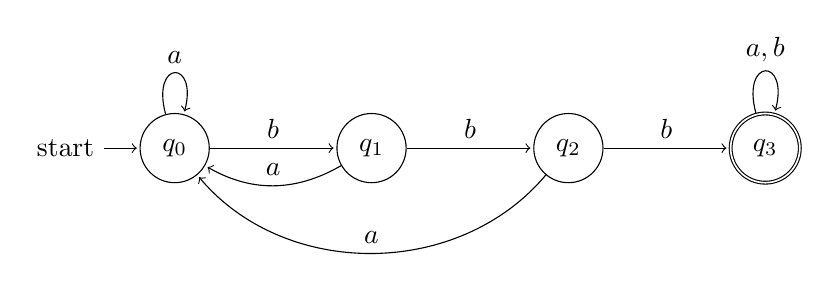
\begin{tikzpicture}[shorten >=1pt,node distance=2.5cm,on grid,auto]
  \node[state, initial] (q0) {$q_0$};
  \node[state] (q1) [right=of q0] {$q_1$};
  \node[state] (q2) [right=of q1] {$q_2$};
  \node[state, accepting] (q3) [right=of q2] {$q_3$};
  \path[->]
    (q0) edge node {$b$} (q1)
         edge [loop above] node {$a$} ()
    (q1) edge node {$b$} (q2)
         edge [bend left] node [swap] {$a$} (q0)
    (q2) edge node {$b$} (q3)
         edge [bend left=50] node [swap] {$a$} (q0)
    (q3) edge [loop above] node {$a,b$} ();
\end{tikzpicture}
\end{center}

\paragraph{Comparison.}
\begin{itemize}
    \item \textbf{(e) and (f) are complements.} Same states and transitions, just with accept/reject swapped. To get the complement of a regular language, flip the accepting states.
    \item \textbf{(c) and (d) share the same structure.} Same transitions, different accepting state. One automaton skeleton, two different languages.
    \item \textbf{(a) vs.\ (b).} For end-patterns (a), the DFA cycles back when the match breaks. For substrings (b), once we find it we're done and sit in the accepting state.
\end{itemize}

\subsubsection{Exploration}

I did research on DFAs to understand them better, here are some interesting things I found.

DFAs can only remember which state they're in. No extra memory, no stack, nothing. That sounds limiting, but it's actually why they're useful.

\paragraph{Where DFAs show up.} Regex engines (\texttt{grep}, Python \texttt{re}, etc.) compile patterns into automata. Compilers use DFAs to break source code into tokens. Even traffic lights and vending machines are basically finite state machines.

\paragraph{Why the limitation is good.} Since DFAs have finite memory, they always finish running, you can always check if two DFAs accept the same language, and you can always shrink a DFA to its smallest form. These are things you lose with stronger models. With a Turing machine, for example, you can't even tell if it will stop running.

\paragraph{DFAs and pure functions.} A pure function always gives the same output for the same input, with no hidden state or side effects. That makes it easy to test and reason about. DFAs work the same way: $\delta(q, a)$ just looks at the current state and symbol, nothing else. You can check every possible behavior because there are only finitely many states. You give up some power but everything is easy to follow.

\subsubsection{Questions}

We showed in Exercise 2 that different-looking DFAs can accept the same language (e.g., the complement pair for $bbb$). Since every regular language has a unique minimal DFA, can you always prove two DFAs are equivalent just by minimizing both and comparing?



















\subsection{Week 2}

\subsubsection{Notes}

This section is optional. 

\subsubsection{Homework}

\textbf{Exercise 2}

Consider two DFAs $\mathcal{B}^{(1)}$ and $\mathcal{B}^{(2)}$ over $\Sigma = \{a, b\}$. We construct their intersection automaton using the product construction.

\paragraph{DFA $\mathcal{B}^{(1)}$.} States $\{p_0, p_1, p_2\}$, start state $p_0$, accepting state $p_0$:

\begin{center}
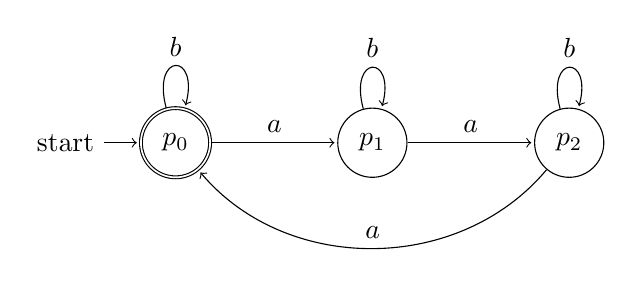
\begin{tikzpicture}[shorten >=1pt,node distance=2.5cm,on grid,auto]
  \node[state, initial, accepting] (p0) {$p_0$};
  \node[state] (p1) [right=of p0] {$p_1$};
  \node[state] (p2) [right=of p1] {$p_2$};
  \path[->]
    (p0) edge node {$a$} (p1)
         edge [loop above] node {$b$} ()
    (p1) edge node {$a$} (p2)
         edge [loop above] node {$b$} ()
    (p2) edge [bend left=50] node [swap] {$a$} (p0)
         edge [loop above] node {$b$} ();
\end{tikzpicture}
\end{center}

\paragraph{DFA $\mathcal{B}^{(2)}$.} States $\{q_0, q_1, q_2\}$, start state $q_0$, accepting state $q_0$:

\begin{center}
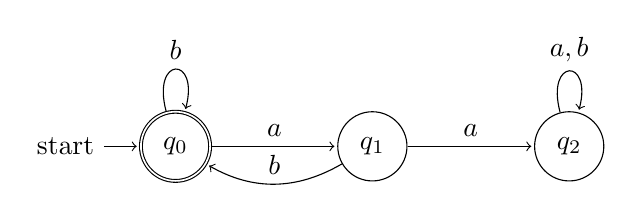
\begin{tikzpicture}[shorten >=1pt,node distance=2.5cm,on grid,auto]
  \node[state, initial, accepting] (q0) {$q_0$};
  \node[state] (q1) [right=of q0] {$q_1$};
  \node[state] (q2) [right=of q1] {$q_2$};
  \path[->]
    (q0) edge node {$a$} (q1)
         edge [loop above] node {$b$} ()
    (q1) edge node {$a$} (q2)
         edge [bend left] node [swap] {$b$} (q0)
    (q2) edge [loop above] node {$a,b$} ();
\end{tikzpicture}
\end{center}

\paragraph{Part 1: Describing the languages.}

\textbf{$L(\mathcal{B}^{(1)})$: Words where the number of $a$'s is divisible by~3.}

Since $b$ self-loops at every state, only $a$'s matter. Reading $a$ cycles $p_0 \to p_1 \to p_2 \to p_0$, and $p_0$ is the only accepting state, so we accept after $0, 3, 6, \ldots$ letters~$a$:
\[
  L(\mathcal{B}^{(1)}) = \{\, w \in \{a,b\}^* : \#_a(w) \equiv 0 \pmod{3} \,\}.
\]

\textbf{$L(\mathcal{B}^{(2)})$: Words where every $a$ is immediately followed by~$b$.}

Reading $a$ from $q_0$ goes to $q_1$, which ``waits'' for a $b$. Getting $b$ returns to $q_0$, but another $a$ traps us in the dead state $q_2$. So every $a$ must have a $b$ right after it, meaning valid words are sequences of $ab$ and $b$ blocks:
\[
  L(\mathcal{B}^{(2)}) = (ab + b)^*.
\]

\paragraph{Part 2: Intersection automaton $\mathcal{B}$.}

Using the product construction, I built $\mathcal{B} = (Q, \Sigma, \delta, (p_0, q_0), F)$ where $Q = \{p_0, p_1, p_2\} \times \{q_0, q_1, q_2\}$ ($9$ states), $\delta((p_i, q_j), x) = (\delta_1(p_i, x),\, \delta_2(q_j, x))$, and $F = \{(p_0, q_0)\}$ since we need both components accepting. Here is the transition table:

\begin{center}
\begin{tabular}{c|cc}
 & $a$ & $b$ \\ \hline
$(p_0, q_0)^{\star}$ & $(p_1, q_1)$ & $(p_0, q_0)$ \\
$(p_0, q_1)$ & $(p_1, q_2)$ & $(p_0, q_0)$ \\
$(p_0, q_2)$ & $(p_1, q_2)$ & $(p_0, q_2)$ \\
$(p_1, q_0)$ & $(p_2, q_1)$ & $(p_1, q_0)$ \\
$(p_1, q_1)$ & $(p_2, q_2)$ & $(p_1, q_0)$ \\
$(p_1, q_2)$ & $(p_2, q_2)$ & $(p_1, q_2)$ \\
$(p_2, q_0)$ & $(p_0, q_1)$ & $(p_2, q_0)$ \\
$(p_2, q_1)$ & $(p_0, q_2)$ & $(p_2, q_0)$ \\
$(p_2, q_2)$ & $(p_0, q_2)$ & $(p_2, q_2)$ \\
\end{tabular}
\end{center}

All nine states are reachable. The six states with $q_0$ or $q_1$ form a hexagonal cycle alternating $a, b, a, b, a, b$. The three $q_2$ states are a dead zone since none of them can reach $(p_0, q_0)$. I drew the dead zone as one dashed node below; see the table for full detail.

\begin{center}
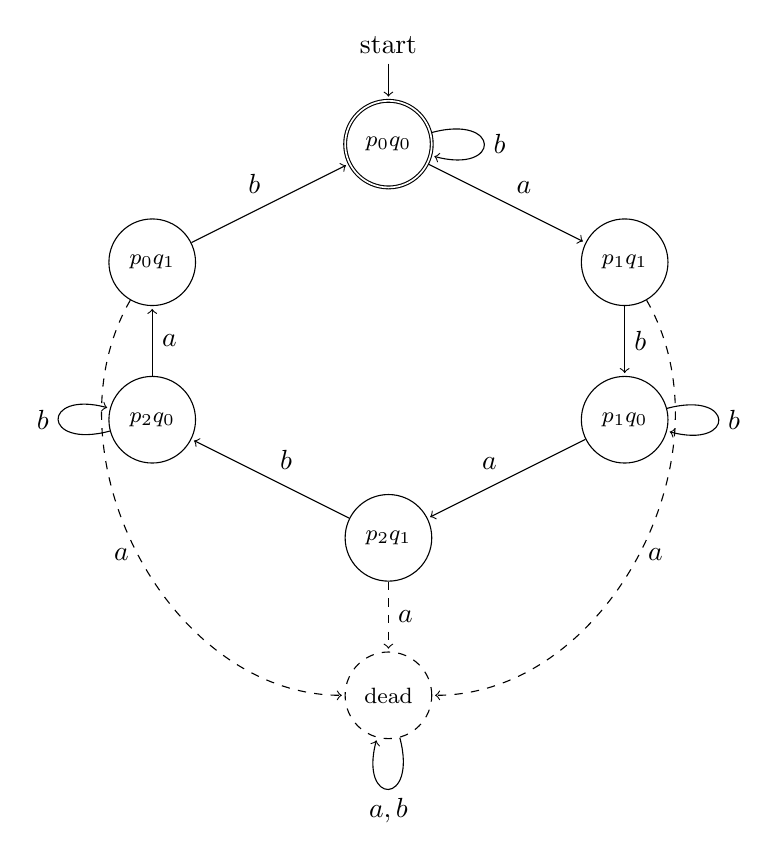
\begin{tikzpicture}[shorten >=1pt, auto,
  every state/.style={minimum size=1.1cm, inner sep=0pt, font=\footnotesize}]
  \node[state, initial above, accepting] (p0q0) at (3,5)   {$p_0 q_0$};
  \node[state]                           (p1q1) at (6,3.5) {$p_1 q_1$};
  \node[state]                           (p1q0) at (6,1.5) {$p_1 q_0$};
  \node[state]                           (p2q1) at (3,0)   {$p_2 q_1$};
  \node[state]                           (p2q0) at (0,1.5) {$p_2 q_0$};
  \node[state]                           (p0q1) at (0,3.5) {$p_0 q_1$};
  \node[state, dashed]                   (dead) at (3,-2)  {\footnotesize dead};
  \path[->]
    % hexagonal cycle (alternating a, b)
    (p0q0) edge node {$a$} (p1q1)
    (p1q1) edge node {$b$} (p1q0)
    (p1q0) edge node [swap] {$a$} (p2q1)
    (p2q1) edge node [swap] {$b$} (p2q0)
    (p2q0) edge node [swap] {$a$} (p0q1)
    (p0q1) edge node {$b$} (p0q0)
    % b self-loops on q0 states
    (p0q0) edge [loop right] node {$b$} ()
    (p1q0) edge [loop right] node {$b$} ()
    (p2q0) edge [loop left]  node {$b$} ()
    % a from q1 states into dead zone
    (p0q1) edge [dashed, out=-120, in=180] node [left] {$a$} (dead)
    (p1q1) edge [dashed, out=-60, in=0] node [right] {$a$} (dead)
    (p2q1) edge [dashed] node [right] {$a$} (dead)
    (dead) edge [loop below] node {$a,b$} ();
\end{tikzpicture}
\end{center}

So we need both conditions: every $a$ followed by $b$, and the number of $a$'s divisible by 3. Since each $a$ lives in an $ab$-block, the number of $ab$-blocks must be a multiple of 3:
\[
  L(\mathcal{B}) = L(\mathcal{B}^{(1)}) \cap L(\mathcal{B}^{(2)})
  = \{\, w \in (ab+b)^* : \text{the number of } ab\text{-blocks is divisible by } 3 \,\}.
\]

\paragraph{Part 3: $L(\mathcal{B}) = L(\mathcal{B}^{(1)}) \cap L(\mathcal{B}^{(2)})$.}

We want to show $\hat\delta((p_0,q_0), w) = (\hat\delta_1(p_0, w),\, \hat\delta_2(q_0, w))$ for any word $w$. By induction on $|w|$:

\emph{Base case.} $w = \varepsilon$: $\hat\delta((p_0,q_0),\varepsilon) = (p_0,q_0) = (\hat\delta_1(p_0,\varepsilon),\, \hat\delta_2(q_0,\varepsilon))$. \checkmark

\emph{Inductive step.} Assume it holds for $w$. For any $a \in \Sigma$:
\begin{align*}
  \hat\delta((p_0,q_0), wa)
    &= \delta\bigl(\hat\delta((p_0,q_0), w),\, a\bigr) \\
    &= \delta\bigl((\hat\delta_1(p_0, w),\, \hat\delta_2(q_0, w)),\, a\bigr)
       && \text{(ind.\ hyp.)} \\
    &= \bigl(\delta_1(\hat\delta_1(p_0, w), a),\;
             \delta_2(\hat\delta_2(q_0, w), a)\bigr)
       && \text{(def.\ of } \delta \text{)} \\
    &= \bigl(\hat\delta_1(p_0, wa),\;
             \hat\delta_2(q_0, wa)\bigr).
\end{align*}

Then $w \in L(\mathcal{B})$ iff we land in $F_1 \times F_2$, iff both components accept, iff $w \in L(\mathcal{B}^{(1)}) \cap L(\mathcal{B}^{(2)})$. \qed

\paragraph{Part 4: $L(\mathcal{B}') = L(\mathcal{B}^{(1)}) \cup \overline{L(\mathcal{B}^{(2)})}$.}

We reuse the same product automaton from Part~2 and just change which states are accepting. Complementing $\mathcal{B}^{(2)}$ flips its accept states: $\overline{F_2} = \{q_1, q_2\}$. For the union we accept when the first component accepts \emph{or} the second rejects:
\[
  F' = \{(p_i, q_j) : p_i \in F_1 \text{ or } q_j \notin F_2\}
     = \{(p_i, q_j) : p_i = p_0 \text{ or } q_j \in \{q_1, q_2\}\}.
\]

That gives $F' = \{(p_0,q_0),\, (p_0,q_1),\, (p_0,q_2),\, (p_1,q_1),\, (p_1,q_2),\, (p_2,q_1),\, (p_2,q_2)\}$. Only $(p_1, q_0)$ and $(p_2, q_0)$ are non-accepting. By the same induction as Part~3, $w \in L(\mathcal{B}')$ iff $\hat\delta_1(p_0,w) \in F_1$ or $\hat\delta_2(q_0,w) \notin F_2$, which is $L(\mathcal{B}^{(1)}) \cup \overline{L(\mathcal{B}^{(2)})}$. \qed

\subsubsection{Exploration}

After some research I noticed that regex tools like \texttt{grep} and Python \texttt{re} have union (\texttt{|}) but no intersection or complement operator. The theory says these operations keep you inside regular languages, but the product construction squares the number of states, so most engines just skip it.

\subsubsection{Questions}

The complement of a DFA is easy (just flip accepting states). Why isn't there an equally simple trick for intersection without building the full product?

























\section{Synthesis}

(approx 1 page, plus references)Section 2 gives you an opportunity to practice "skill drill" and to explore the material in more depth. The purpose of this section is to synthesize the knowledge you gained. Since Programming Languages is a wide field, it may be appropriate to focus on a particular topic of your choice. 

We suggest the following timeline. Week 5-8: Decide on a topic and discuss it with your instructor in the office hours. Write a summary email to your instructor after office hours, including the feedback you got with further reflection and planning. Week 9-12: Write a draft of your synthesis and discuss it with your instructor during office hours. Again, write a summary email to your instructor after office hours, including the feedback you got with further reflection and planning. The final version of the Synthesis is due with the rest of the final report.

Here are some example titles you can think of for this section:

\begin{itemize}
\item \textbf{Standard Academic Titles}
  \begin{itemize}
  \item ``Synthesis and Reflection''
  \item ``Integration of Concepts''
  \item ``Synthesis of Learning''
  \item ``Critical Synthesis''
  \end{itemize}

\item \textbf{Algorithm Analysis Focus}
  \begin{itemize}
  \item ``The Core of the Code: A Personal Synthesis''
  \item ``Connecting the Dots: From Theory to Practice''
  \item ``The Big Picture: Algorithm Analysis in Context''
  \item ``Principles of Problem-Solving''
  \end{itemize}

\item \textbf{Concept-Focused Titles}
  \begin{itemize}
  \item ``Beyond the Code: Understanding the Essence of Algorithms''
  \item ``How long is too long? A Case Study in Complexity Theory''
  \item ``Principles of Computation''
  \item ``Abstract Machines for Concrete Problems''
  \item ``Is there an Algorithm for this? On (Un)Decidability''
  \end{itemize}

\item \textbf{Process-Focused Titles}
  \begin{itemize}
  \item ``My Journey Through Algorithm Analysis''
  \item ``From Implementation to Understanding''
  \item ``Building Mental Models of Practical Problems''
  \item ``Discovering the Foundations behind Algorithms''
  \end{itemize}
\end{itemize}


\section{Evidence of Participation}
\section{Conclusion}\label{conclusion}

(approx 400 words) A critical reflection on the content of the course. Step back from the technical details. How does the course fit into the wider world of software engineering? What did you find most interesting or useful? What improvements would you suggest?

\begin{thebibliography}{99}
\bibitem[BLA]{bla} Author, \href{https://en.wikipedia.org/wiki/LaTeX}{Title}, Publisher, Year.
\end{thebibliography}

\end{document}
